\documentclass[12pt,a4paper]{report}

% --- Packages ---
\usepackage[utf8]{inputenc}
\usepackage[T1]{fontenc}
\usepackage{graphicx}
\usepackage{geometry}
\geometry{a4paper, margin=1in, headheight=15pt, top=1.2in, bottom=1.2in}
\usepackage{hyperref}
\usepackage{float}
\usepackage{caption}
\usepackage{titlesec}
\usepackage{fancyhdr}
\usepackage{xcolor}
\usepackage{listings}
\usepackage{setspace}

\onehalfspacing

% --- Styling ---
\hypersetup{
    colorlinks=true,
    linkcolor=blue,
    filecolor=magenta,      
    urlcolor=cyan,
    pdftitle={eSim Fellowship Comprehensive Project Report},
    hypertexnames=false,
}

\definecolor{codegreen}{rgb}{0,0.6,0}
\definecolor{codegray}{rgb}{0.5,0.5,0.5}
\definecolor{codepurple}{rgb}{0.58,0,0.82}
\definecolor{backcolour}{rgb}{0.95,0.95,0.92}

\lstdefinestyle{mystyle}{
    backgroundcolor=\color{backcolour},   
    commentstyle=\color{codegreen},
    keywordstyle=\color{magenta},
    numberstyle=\tiny\color{codegray},
    stringstyle=\color{codepurple},
    basicstyle=\ttfamily\small,
    breakatwhitespace=false,         
    breaklines=true,                 
    captionpos=b,                    
    keepspaces=true,                 
    numbers=left,                    
    numbersep=5pt,                  
    showspaces=false,                
    showstringspaces=false,
    showtabs=false,                  
    tabsize=2
}
\lstset{style=mystyle}

% --- Header/Footer ---
\pagestyle{fancy}
\fancyhf{}
\rhead{\thepage}
\lhead{eSim Summer Fellowship Report}
\cfoot{}

\begin{document}

% ======================================================
% TITLE PAGE
% ======================================================
\begin{titlepage}
    \centering
    
    
\includegraphics[width=0.7\textwidth]{figures/Logo.png} \\[1cm]
    
    {\Huge \textbf{eSim Summer Fellowship 2026}} \\[0.8cm]
    
    {\normalsize On} \\[0.5cm]
    {\Large \textbf{GUI Enhancements in Tool Manager and}} \\[0.2cm]
    {\Large \textbf{KiCad Frontend and Documentation Refactor}} \vfill
    
    {\normalsize Submitted by} \\[0.3cm]
    {\large \textbf{MAUSAM KAR}} \\[0.1cm]
    {\normalsize Department of Computer Science and Engineering} \\[0.1cm]
    {\normalsize VIT Bhopal University} \vfill
    
    {\normalsize Under the guidance of} \\[0.3cm]
    {\large \textbf{Prof. Prabhu Ramachandran}} \\[0.1cm]
    {\normalsize Principal Investigator} \\[0.1cm]
    {\normalsize Department of Aerospace Engineering} \\[0.1cm]
    {\normalsize Indian Institute of Technology Bombay} \vfill
    
    {\normalsize July 5, 2026}
\end{titlepage}

\pagenumbering{roman}
\setcounter{page}{1}

% ======================================================
% DECLARATION
% ======================================================
\chapter*{Declaration}
\addcontentsline{toc}{chapter}{Declaration}
I hereby declare that the project report titled \textbf{"GUI Enhancements in Tool Manager and KiCad Frontend and Documentation Refactor"}, submitted by me for the eSim Summer Fellowship 2026, is a record of genuine work carried out by me as part of my academic and technical work at the Department of Computer Science and Engineering, VIT Bhopal University.

The work presented in this report has not been previously submitted for any other purpose. All sources, both primary and secondary, have been duly acknowledged.



% ======================================================
% ACKNOWLEDGEMENT
% ======================================================
\chapter*{Acknowledgement}
\addcontentsline{toc}{chapter}{Acknowledgement}
I express my sincere gratitude to \textbf{Prof. Prabhu Ramachandran} for providing me with the opportunity to be part of the \textbf{FOSSEE} internship program and for his continued efforts in promoting open-source engineering tool development. His leadership and vision have been instrumental in fostering meaningful student participation in the open-source ecosystem.

I also acknowledge \textbf{Prof. Kannan M. Moudgalya} for his foundational role in establishing and strengthening the \textbf{FOSSEE} initiative. His contributions to open-source education and the development of the \textbf{FOSSEE} fellowship framework have been pivotal in creating the academic and organisational platform through which this internship was undertaken.

My sincere appreciation extends to my mentor, \textbf{Sumanto Kar}, for his continual support, technical guidance, and encouragement throughout the duration of this project. His insights and feedback played a key role in refining ideas, overcoming challenges, and ensuring timely completion of the tasks assigned to me.

I would also like to thank my internal mentors, \textbf{Mr. Varad Patil} and \textbf{Ms. Shanthi Priya K} for their valuable guidance, coordination, and technical inputs during the internship. Their mentorship contributed significantly to the clarity, progress, and successful execution of the work.

This internship has been an enriching learning experience, allowing me to work closely with open-source EDA tools, focusing on documentation refactoring, GUI enhancements in the Automated Tool Manager, and \textbf{KiCad} frontend development. The knowledge acquired during this period will undoubtedly support my future academic and professional pursuits.

I would also like to thank the entire \textbf{FOSSEE} team for their coordination, assistance, and timely interactions at various stages of this work. Their collective efforts ensured smooth workflow, resource accessibility, and effective project execution.

Finally, I am also thankful to the Department of Computer Science and Engineering at \textbf{VIT Bhopal University} for maintaining an environment conducive to learning and innovation, and for encouraging research and development activities among its students.



% ======================================================
% ABSTRACT
% ======================================================
\chapter*{Abstract}
\addcontentsline{toc}{chapter}{Abstract}
This comprehensive report documents the extensive contributions made during the eSim Summer Fellowship 2026. The primary focus of this intensive fellowship period was the complete overhaul of the core repository's documentation architecture and the deep graphical enhancement of the Automated Tool Manager's user interface.

Electronic Design Automation (EDA) tools like eSim require robust, accessible documentation to foster open-source growth. The documentation overhaul replaced basic legacy text with a dynamic, highly organized markdown architecture. This involved integrating live-updating contribution metrics, professional status shields, and a detailed Mermaid-based architectural diagram that visually maps the entire eSim ecosystem.

Concurrently, the GUI of the integrated Tool Manager required significant refactoring. Early iterations suffered from severe typography overlaps, lack of responsive design on smaller displays, and critical rendering failures triggered by OS-level dark mode overrides on Windows. By implementing explicit stylesheet enforcements, dynamic \texttt{QScrollArea} wrappers, and modernized spacing metrics, the interface was successfully transformed into a polished, production-ready system.

This report provides an in-depth analysis of these implementations, presenting the exact codebase modifications, architectural designs, and the numerous technical challenges overcome to achieve the final release candidate.

\vskip 1cm
\textbf{Keywords:} eSim, Markdown Architecture, PyQt6, UI/UX Refactoring, Dark Mode Overrides

\newpage
\begin{singlespace}
\tableofcontents
\end{singlespace}
\newpage
\listoffigures
\pagenumbering{arabic}
\setcounter{page}{1}

% ======================================================
% CHAPTER 1: INTRODUCTION
% ======================================================
\chapter{Introduction}
\section{Background of eSim and FOSSEE}
The Free and Open Source Software for Education (FOSSEE) project at IIT Bombay has long championed the democratization of technical education through open-source software. At the forefront of this initiative is eSim, an advanced Electronic Design Automation (EDA) tool designed for circuit design, simulation, and printed circuit board (PCB) routing.

eSim acts as an orchestration layer, seamlessly integrating powerful underlying open-source utilities such as KiCad for schematic capture and PCB layout, and Ngspice for mixed-level/mixed-signal circuit simulation. By abstracting the complexities of these individual tools, eSim provides a unified, cohesive environment suitable for both academic instruction and professional engineering.

\section{Initial Exploration and Identifying Bottlenecks}
My journey with the eSim platform began on May 18, 2026, with an initial orientation and exploration phase. Over the first week, I immersed myself in the project by watching tutorials and selecting my major and minor tasks. I joined the Zulip channels and spent significant time analyzing the commit history and workflows of prior interns to understand the project's pulse. During these early discussions with fellow peers and mentors, I deeply explored the eSim architecture through the official FOSSEE documentation. 

By the end of May, I had successfully forked and cloned the repository, set up my local development environment, resolved project dependencies, and built the eSim project locally. It was during this hands-on exploration of the KiCad frontend source code and the Tool Manager that I noticed significant gaps. Despite its powerful backend capabilities, I found that the documentation was not up to the mark for an open-source project of this scale. The primary documentation lacked visual hierarchy, failed to provide immediate project status, and did not offer a clear architectural map. Simultaneously, the newly integrated Tool Manager exhibited severe graphical user interface (GUI) instability. On Windows machines, OS-level dark mode themes caused stylesheets to bleed, rendering text invisible, and dynamic resizing often obscured critical installation controls.

\section{Methodology and Fellowship Timeline}
Realizing that these unpolished touchpoints would hinder community adoption, I decided to take immediate action. From June 1 onwards, I began a systemic overhaul. I first analyzed and configured the Dockerfile to containerize the Tool Manager environment. I then performed a comprehensive analysis of the entire codebase and prepared an improvement plan for restructuring the README. Between June 3 and June 6, I expanded the README into a comprehensive technical guide spanning over 800 lines. This involved designing detailed architectural diagrams, workflow illustrations, and component relationship visualizations to significantly improve project understanding.

Following the documentation overhaul, I shifted my focus to the GUI. On June 8, I implemented an initial UI overhaul but received critical team feedback that the UI should be improved incrementally rather than replaced entirely. Embracing this feedback, I meticulously reviewed the existing implementation and divided the work into modular fixes in collaboration with my peers, Akanksha and Yash. By mid-June, I successfully investigated and resolved section-overlapping issues by implementing a dynamic scroll area for the Quick Setup tab. I systematically enhanced the Individual Tools table by adjusting cell padding and row heights for maximum readability. 

Finally, towards the end of June, I tackled the most persistent rendering bugs. I applied explicit light-themed stylesheets to the Uninstall Tools dialog, fixing the dark color bleeding, and completely restyled the installation progress console. With the major tasks complete, I transitioned into minor tasks, evaluating the KiCad frontend UI theme and documenting a comprehensive implementation plan for future bug fixes, culminating in a final actionable report presented at the project review.

To provide a structured overview of the technical processes followed during this project, the methodology is divided into five key phases:
\begin{itemize}
    \item \textbf{Systematic Codebase Analysis and Diagnostics:} Prior to implementing any codebase modifications, a comprehensive analysis of the repository was conducted. This involved running static analysis tools, evaluating runtime memory footprints of the Tool Manager, and documenting UI rendering failures on various Windows versions (Windows 10 and 11) under dark and light themes.
    \item \textbf{Dockerized Environment Development:} To guarantee isolation and cross-platform consistency during development and testing, a containerized setup was established using Docker. This allowed the simulated installation environments (including MSYS2/MinGW virtual roots) to be tested without contaminating the host operating system's environment variables.
    \item \textbf{Documentation Restructuring Workflow:} The restructuring of the README and creation of the CONTRIBUTING guidelines followed a modular approach. This started with mapping folder hierarchies, creating raw SVG assets, writing the JSON query structures for dynamic API badges (via shields.io), and rendering the system layout in Mermaid.js syntax.
    \item \textbf{UI/UX Refactoring and Regression Testing:} The GUI refactoring was executed iteratively. First, the spacing variables and stylesheet strings were extracted into central constants. Then, layout components (such as \texttt{QTableWidget}, \texttt{QScrollArea}, and custom dialogs) were refactored for padding, margins, and layout constraint policies. Crucially, manual regression testing was performed after each UI modification to ensure compatibility across high-DPI displays and system theme toggles.
    \item \textbf{KiCad Frontend Debugging and Path Parsing Analysis:} The minor tasks were executed by tracing stack traces in the KiCad-to-Ngspice converter components and testing dialog geometry under PyQt6 constraints. Path-escaping mechanisms were updated to prevent space-character splitting issues in directory locations on Windows environments.
\end{itemize}

The cumulative progress and progression of these tasks throughout the fellowship timeline are illustrated in Figure~\ref{fig:worksheet}.

\begin{figure}[H]
    \centering
    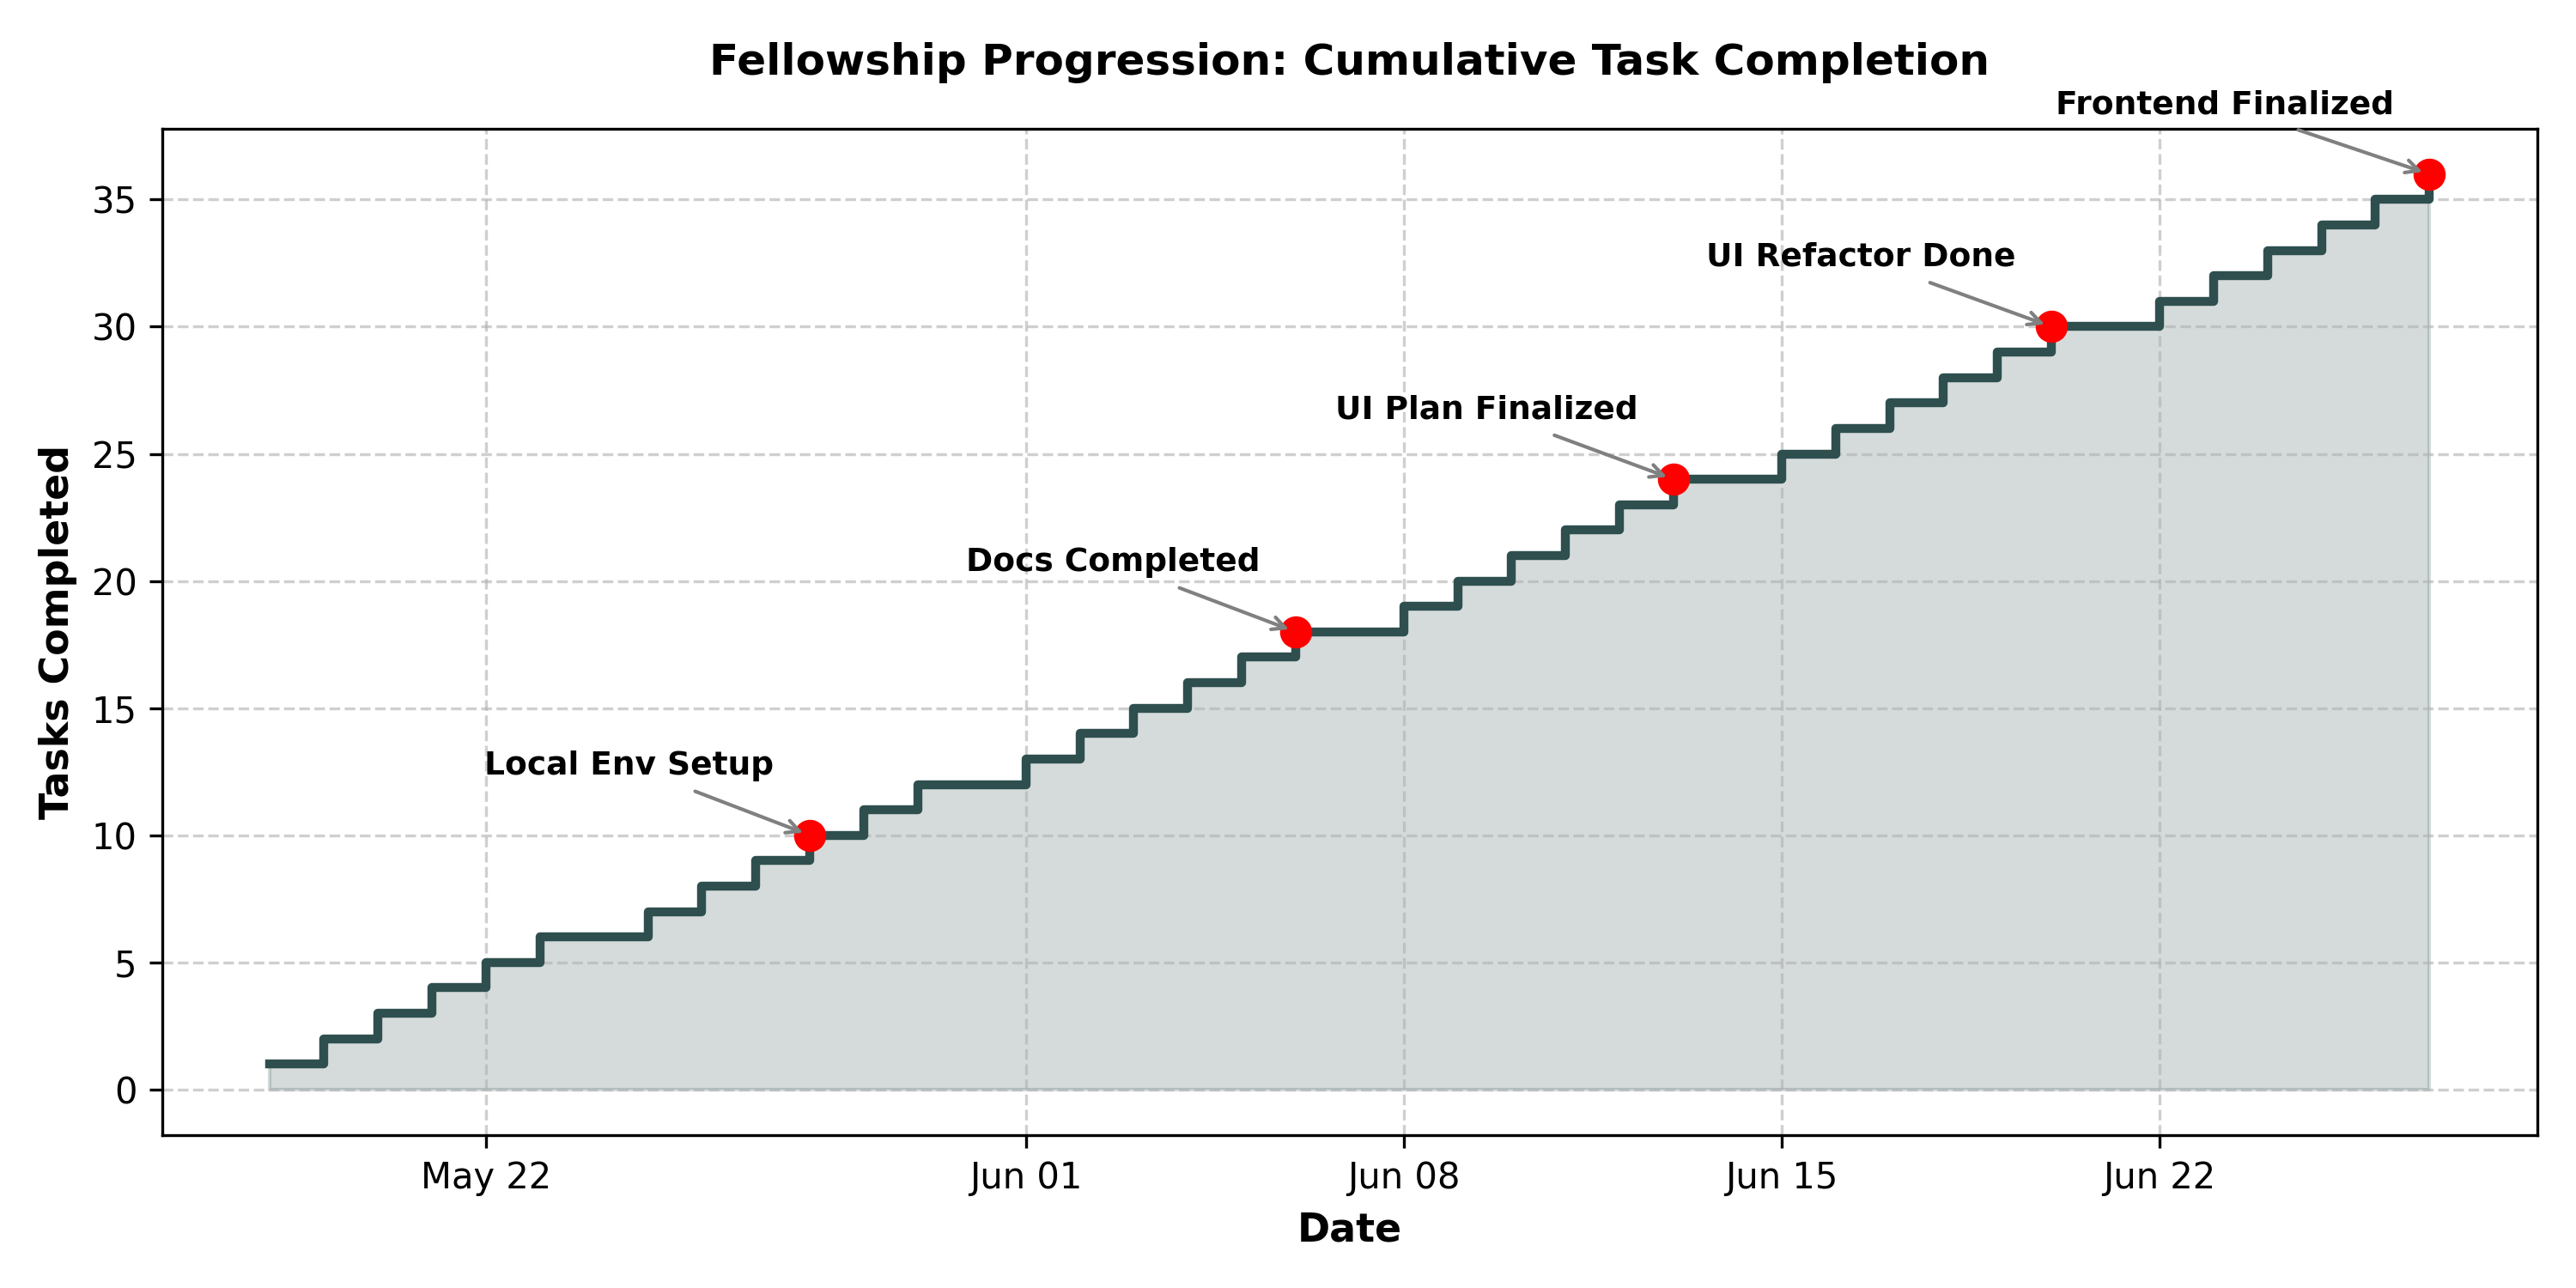
\includegraphics[width=0.9\textwidth]{figures/worksheet_progress.png}
    \caption{Fellowship Progression: Cumulative Task Completion Timeline}
    \label{fig:worksheet}
\end{figure}

\section{Report Structure}
This comprehensive document spans several codesigned and detailed chapters to provide a meticulous breakdown of this technical journey, serving as both a record of achievement and a future guide for eSim developers. 

\begin{itemize}
    \item \textbf{Chapter 2: System Architecture Documentation} -- Dives deep into the architectural documentation overhaul, specifically focusing on the translation of complex backend structures into accessible, auto-rendering Mermaid diagrams. It discusses the rationale behind visual documentation, outlines the exact syntax and topology of the implemented flowchart, and details the resolution of rendering bugs in GitHub's markdown renderer.
    \item \textbf{Chapter 3: Documentation Overhaul \& Live Metrics} -- Explores the broader repository-wide documentation overhaul. This includes the strategic integration of live, self-updating GitHub API metrics, the complete restructuring of the README and CONTRIBUTING guidelines, the implementation of dynamic HTML contributor walls using GitHub APIs, and the integration of security and licensing protocols (specifically GPL v3.0 compliance and security vulnerability reporting guidelines).
    \item \textbf{Chapter 4: Advanced GUI Enhancements \& Refactoring} -- Shifts focus to the core software component, providing a deep technical analysis of the GUI enhancements implemented in the Automated Tool Manager. Complete with visual proofs of before-and-after states, it details the engineering challenges overcome to deliver a modern, cross-platform interface resistant to OS-level style overrides, layout overlaps, and dark theme background contrast bleeding.
    \item \textbf{Chapter 5: Minor Task: KiCad Frontend Analysis \& Bug Fixes} -- Details the minor tasks completed during the fellowship, focusing on the investigation and resolution of layout issues, API migration regressions (PyQt5 to PyQt6 enum mapping), and path resolution bugs within the KiCad frontend dialogs and its converters.
    \item \textbf{Chapter 6: Version Control \& Deployment Workflows} -- Outlines the version control, continuous integration integrity, and deployment workflows observed during the fellowship. It documents the atomic commit strategy (following Conventional Commits), branch management protocols, and future automated release workflows utilizing GitHub Actions and automatic documentation generation.
    \item \textbf{Chapter 7: Conclusion and Future Work} -- Concludes the report with reflections on the invaluable skills acquired, the overall impact on the eSim platform, and proposals for future technical work (such as AI-powered debugging integration, Dockerized runtime packages, and pytest-qt automated UI test suites).
\end{itemize}

% ======================================================
% CHAPTER 2: ARCHITECTURE DOCUMENTATION
% ======================================================
\chapter{System Architecture Documentation}
\section{Role of Architectural Diagrams in Open Source}
For a project as expansive as eSim—which bridges Python-based GUIs with C++ backend simulators—onboarding new developers is a daunting task. Without a high-level map, contributors often struggle to understand how modifications in the \texttt{modelEditor} might impact the \texttt{ngspiceSimulation} engine. 

To solve this, I spearheaded the creation of a definitive \texttt{ARCHITECTURE.md} document, anchored by a dynamic, code-driven diagram using Mermaid.js.

\section{Implementing the Mermaid Diagram}
Mermaid.js was selected because it allows diagrams to be version-controlled alongside the code, eliminating the need for external image editing software. The diagram was designed using a \texttt{flowchart LR} (Left-to-Right) topology to illustrate the data pipeline from user input to simulation output.

\subsection{Mermaid Source Code Implementation}
The following is the exact Mermaid code I authored to map the eSim ecosystem:

\begin{lstlisting}
flowchart LR
    %% Core System Nodes
    User([End User])
    eSim[eSim Main App]
    ToolManager[Automated Tool Manager]
    
    %% Functional Modules
    subgraph Schematic & Design
        KiCad[KiCad (Schematic)]
        ModelEditor[Model Editor]
        Subcircuit[Subcircuit Builder]
    end
    
    subgraph Simulation & Analysis
        kicadToNgspice[Netlist Converter]
        Ngspice[Ngspice Engine]
        Plotting[Matplotlib Waveforms]
    end
    
    %% Integrations
    subgraph External Integrations
        Makerchip[Makerchip Cloud]
        NgVeri[NgVeri Verilog]
    end
    
    %% Connections
    User --> eSim
    eSim -.-> ToolManager
    ToolManager --> KiCad
    ToolManager --> Ngspice
    
    eSim --> KiCad
    KiCad -- Netlist --> kicadToNgspice
    kicadToNgspice --> Ngspice
    Ngspice -- Data --> Plotting
    
    eSim --> ModelEditor
    eSim --> Subcircuit
    ModelEditor -.-> Ngspice
    
    eSim --> Makerchip
    Makerchip --> NgVeri
    NgVeri --> Ngspice
\end{lstlisting}

\subsection{Issues Faced: Mermaid Rendering and Complexity}
Creating this diagram was not without challenges. Initially, representing the bidirectional relationship between the Tool Manager and the external dependencies caused the Mermaid rendering engine in GitHub to cross edges violently, resulting in a "spaghetti" visual.

\textbf{Resolution:} To resolve this, I implemented \texttt{subgraph} groupings to isolate functional domains (e.g., \texttt{Schematic \& Design} vs. \texttt{Simulation \& Analysis}). I also utilized dotted links (\texttt{-.->}) to distinguish administrative connections (like the Tool Manager installing KiCad) from direct data flow (like KiCad passing a Netlist to Ngspice). This strict semantic separation forced the rendering engine to align the nodes cleanly.

\begin{figure}[H]
    \centering
    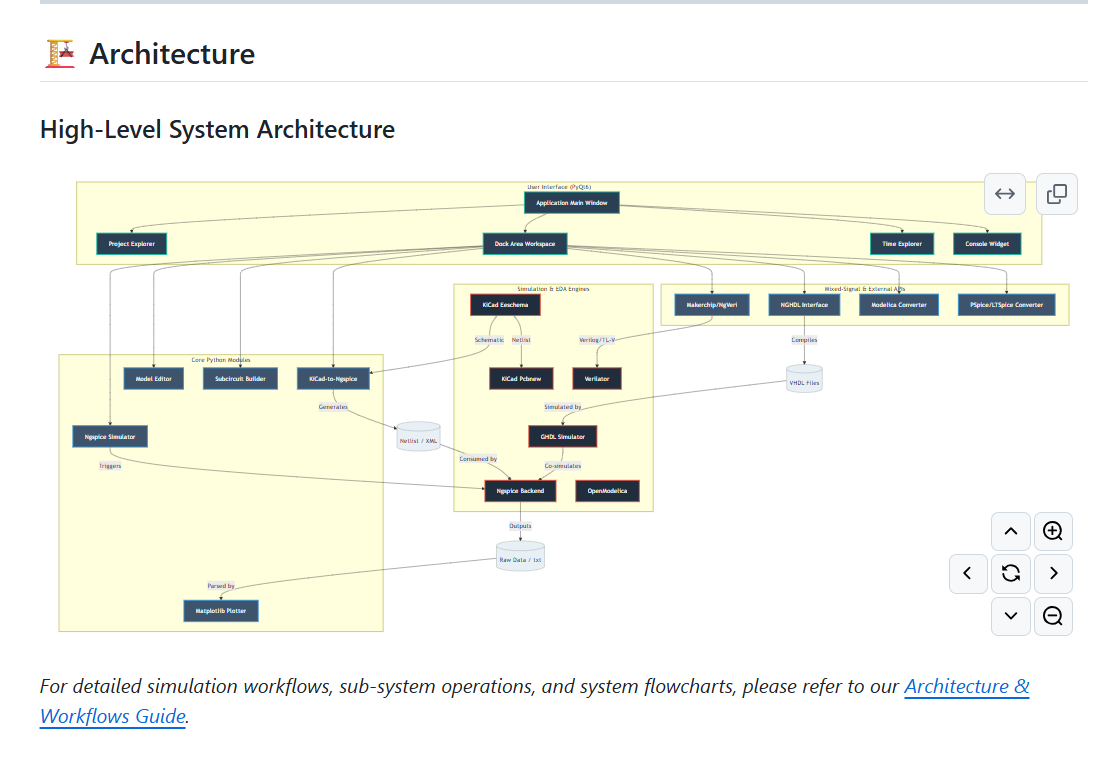
\includegraphics[width=0.9\textwidth]{figures/architecture_diagram.png}
    \caption{System Architecture Diagram}
    \label{fig:mermaid_render}
\end{figure}



% ======================================================
% CHAPTER 3: DOCUMENTATION ENHANCEMENTS
% ======================================================
\chapter{Documentation Overhaul \& Live Metrics}

\section{README.md Restructuring and Style Enhancements}
The repository's primary landing document, \texttt{README.md}, serves as the initial point of contact for external developers and users. Prior to the overhaul, the document consisted of unstructured, dense text blocks lacking visual hierarchy and immediate clarity. To address this, the documentation was refactored to align with modern open-source standards, prioritizing scannability, visual appeal, and concise information delivery.

\subsection{Dynamic Status Badges}
To enhance visual professionalism and provide immediate project metadata, dynamic status badges generated via \texttt{shields.io} were integrated at the header of the document. These badges display critical project attributes, such as Python version compatibility, licensing terms, and the real-time count of open issues and pull requests. By linking these badges to the GitHub API, the project status remains self-updating, offering contributors a live, transparent snapshot of repository activity.

\begin{figure}[H]
    \centering
    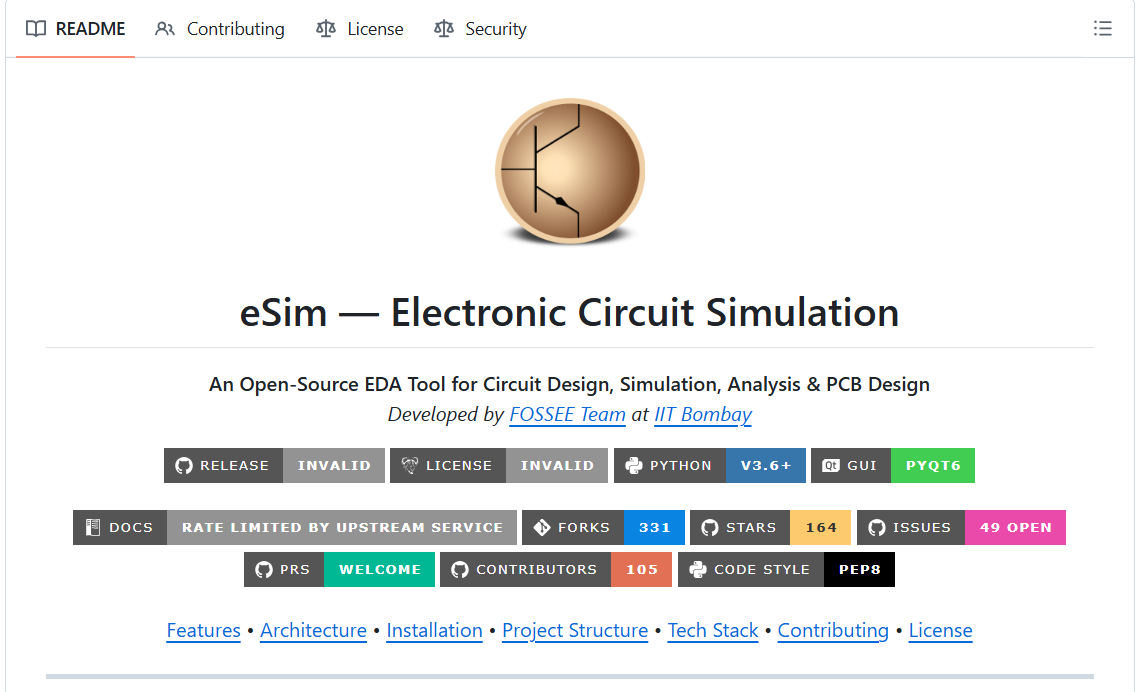
\includegraphics[width=0.9\textwidth]{figures/readme_badges.png}
    \caption{Screenshot of the new README layout featuring live GitHub API badges}
    \label{fig:readme_badges}
\end{figure}

\subsection{Directory Structure and Repository Mapping}
Navigating a complex codebase can introduce substantial onboarding friction for new contributors. To mitigate this, a comprehensive directory mapping was introduced using a hierarchical tree structure. This directory map provides an immediate overview of the repository's functional components. For example, developers seeking to modify backend conversion scripts versus frontend user interfaces can instantly locate their target directories. This structured overview reduces lookup times, minimizes the risk of accidental modifications to unrelated modules, and establishes a standardized blueprint for future directory expansions.

\begin{figure}[H]
    \centering
    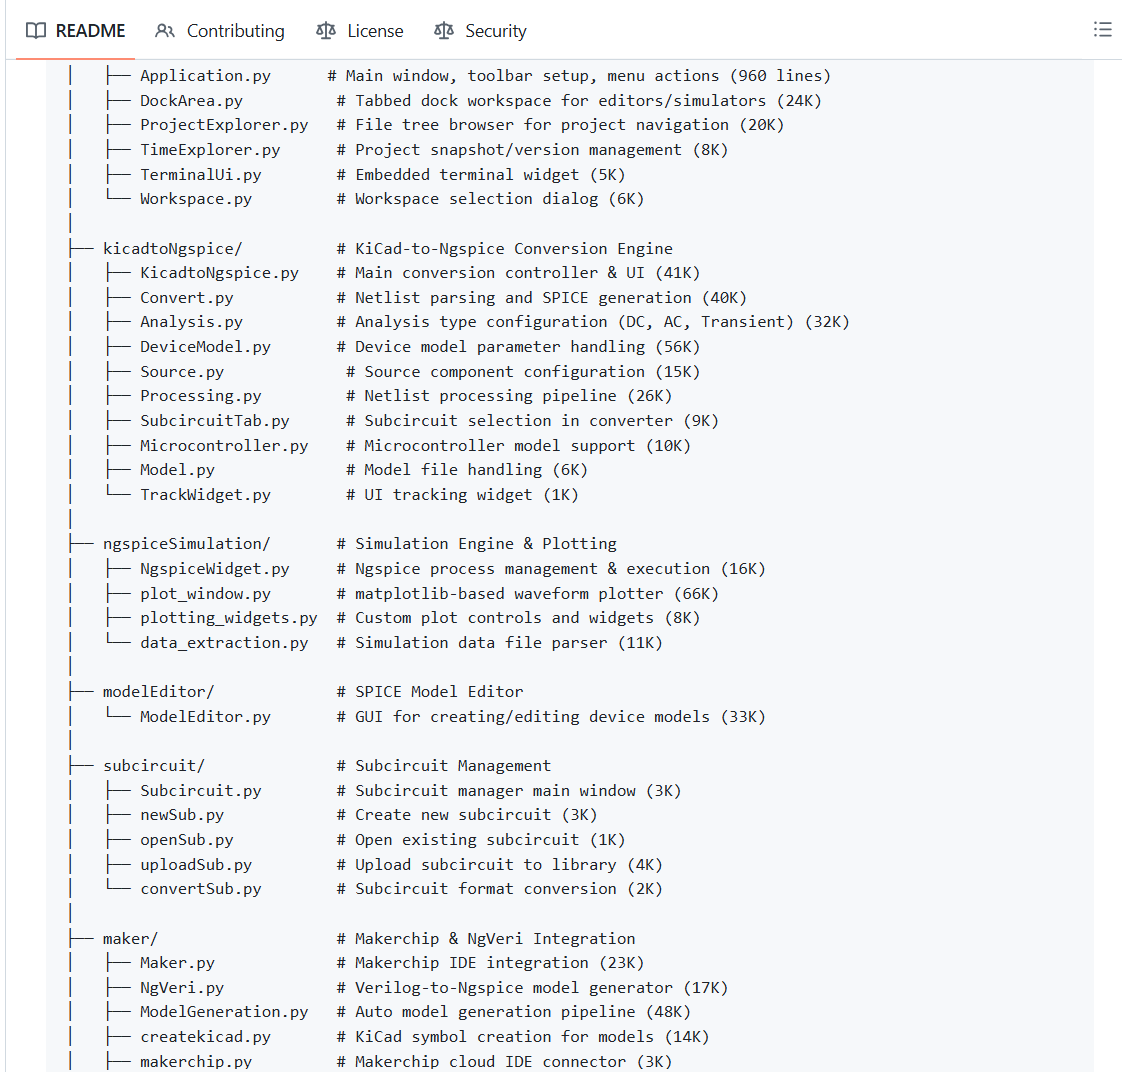
\includegraphics[width=0.9\textwidth]{figures/readme_folder_hierarchy.png}
    \caption{Screenshot of the Detailed Folder Hierarchy section in the README}
    \label{fig:readme_folder_hierarchy}
\end{figure}

\subsection{Tabulated Installation and Feature Reference}
The original documentation relied on dense prose to explain system features, installation steps, and cross-platform dependencies, which reduced readability. To streamline information retrieval, this content was consolidated into structured tables. Tabulating the setup procedures and dependency requirements allows users to quickly identify commands specific to their host operating system (e.g., Linux, Windows, or macOS). This tabular layout facilitates direct command execution, thereby reducing user installation errors and enhancing the general usability of the eSim platform.

\begin{figure}[H]
    \centering
    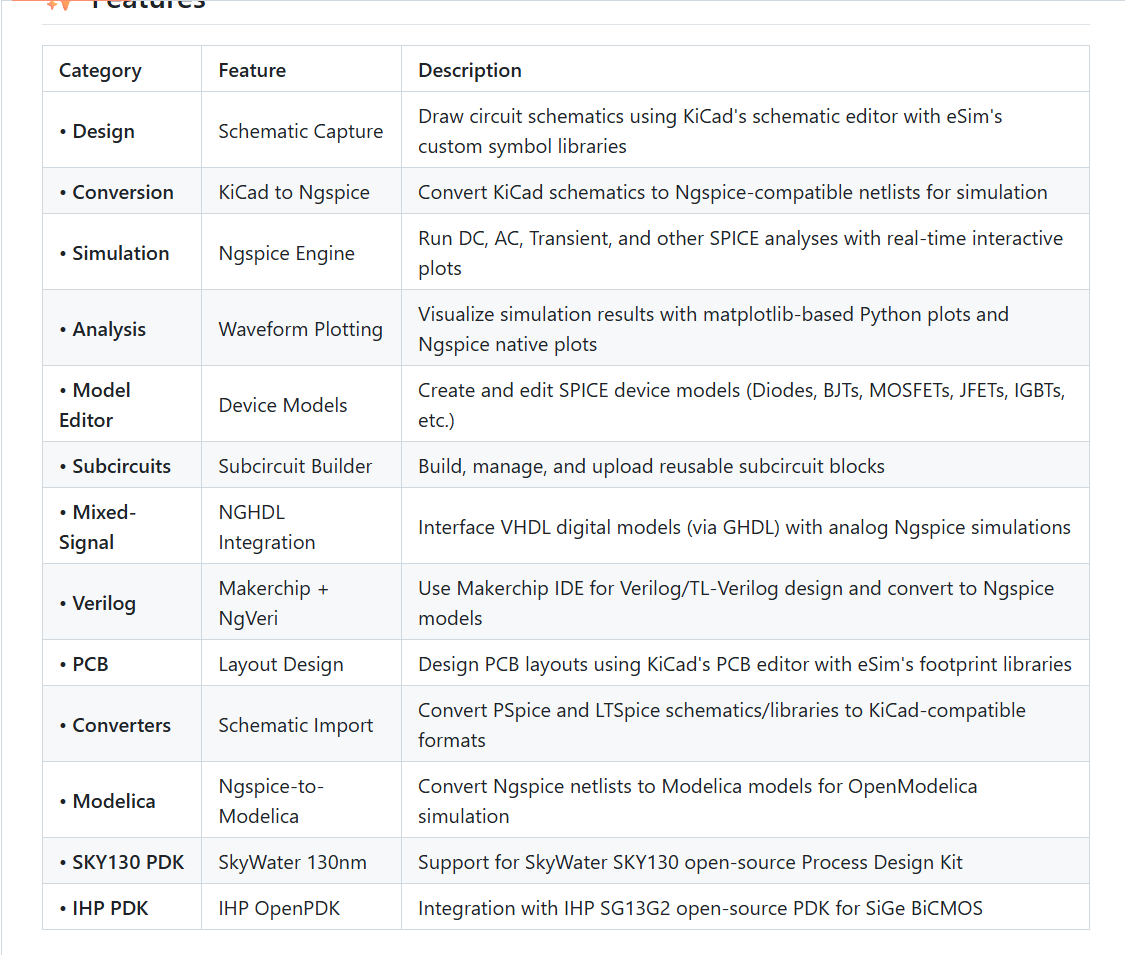
\includegraphics[width=0.9\textwidth]{figures/readme_tabular.png}
    \caption{Screenshot showing the tabular format used for installation and features}
    \label{fig:readme_tabular}
\end{figure}

\section{The Structured CONTRIBUTING.md Guidelines}
The original contribution guidelines were brief and did not provide sufficient detail. To establish a rigorous standard for community contributions, the \texttt{CONTRIBUTING.md} file was expanded into a comprehensive developer guide. This document outlines the coding standards, branch management strategies, and pull request workflows required to maintain codebase integrity.

\subsection{Dynamic Contributor Profile Integration}
One of the most significant additions was the dynamic contributor recognition section in the README and CONTRIBUTING files. I utilized raw HTML tables combined with the GitHub avatar API to create a live-updating contributor wall featuring circular profile views.

\begin{lstlisting}[language=HTML]
<table align="center" style="border:none;">
  <tr>
    <td align="center" width="250" style="border:none;">
      <a href="https://github.com/Eyantra698Sumanto" style="text-decoration:none;">
        <img src="https://github.com/Eyantra698Sumanto.png" width="120" height="120" style="border-radius:50%;" alt="Sumanto Kar"/><br/>
        <b>Sumanto Kar</b>
      </a><br/>
      <sub>Lead Maintainer</sub>
    </td>
  </tr>
</table>
\end{lstlisting}

By explicitly injecting \texttt{border-radius} and \texttt{width} tags, I achieved a responsive, circular aesthetic that automatically updates whenever a new contributor merges a pull request.

\begin{figure}[H]
    \centering
    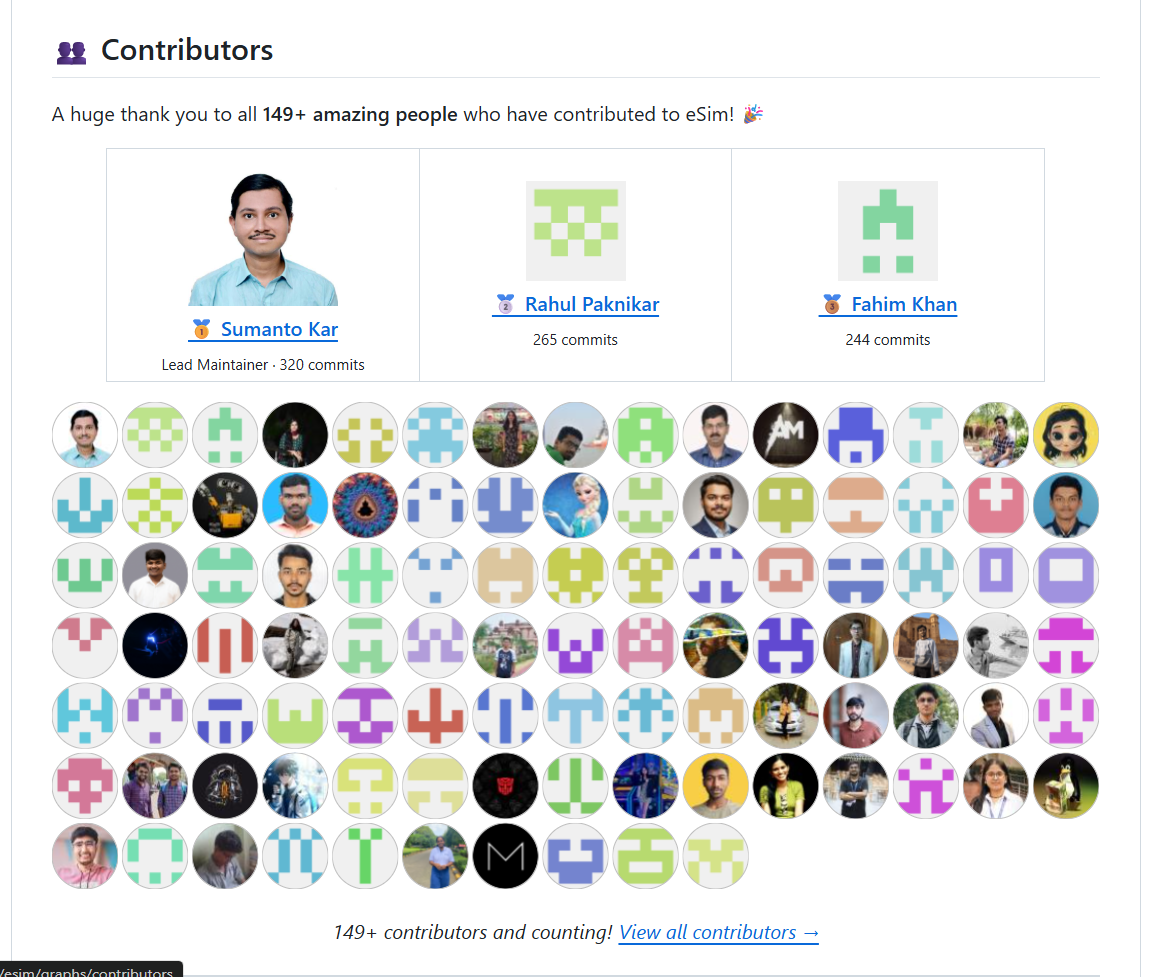
\includegraphics[width=0.9\textwidth]{figures/contrib_live_circular.png}
    \caption{Screenshot of the Live Updating Circular Contributor Profiles}
    \label{fig:contrib_live_circular}
\end{figure}

\subsection{Visualizing Contribution History and Activity}
To illustrate project activity and historical engagement, dynamic contribution history graphs were embedded directly into the documentation. These elements render commit frequencies over time, offering a clear visual representation of repository health and maintainer momentum.

\begin{figure}[H]
    \centering
    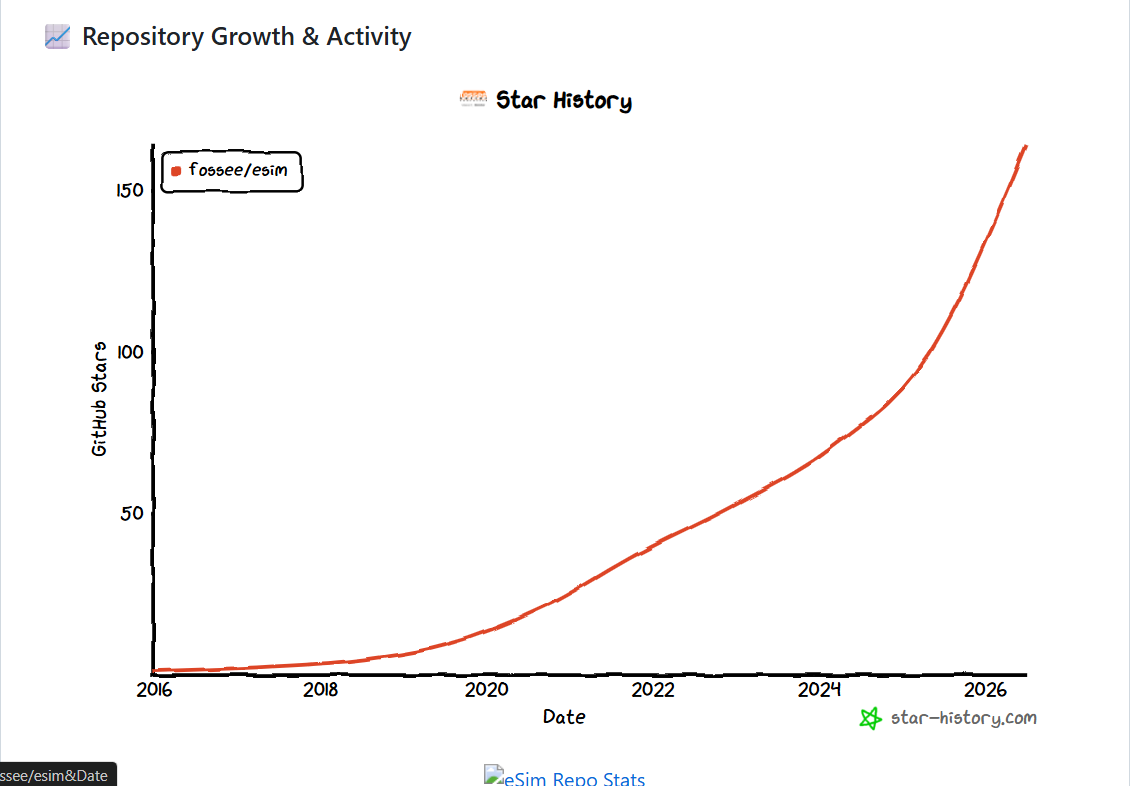
\includegraphics[width=0.9\textwidth]{figures/contrib_graph.png}
    \caption{Screenshot of the Contribution Over Time Graph in the contributing section}
    \label{fig:contrib_graph}
\end{figure}

\section{Security and Licensing Enhancements}
Finally, to elevate the repository to meet modern enterprise open-source standards, I recognized that security protocols and licensing terms were insufficiently documented. I extracted the brief, buried mentions of these topics and heavily expanded them into dedicated, highly visible sections. 

Most importantly, I authored a dedicated \texttt{SECURITY.md} file, a crucial component for any production-level open-source project. This document explicitly outlines the project's responsible vulnerability reporting policies, providing security researchers with a clear, private channel to report exploits before they are publicly disclosed. This ensures the safety of the entire eSim user base against potential zero-day vulnerabilities in the tool ecosystem.

Furthermore, I clarified the intricate GNU GPL v3.0 licensing constraints that govern the repository. By explicitly spelling out what users can and cannot do, I ensured that any derivative works, commercial applications, or academic distributions are properly legally structured and compliant with open-source regulations. This removes legal ambiguity, protecting both the core maintainers and the community contributors.

\begin{figure}[H]
    \centering
    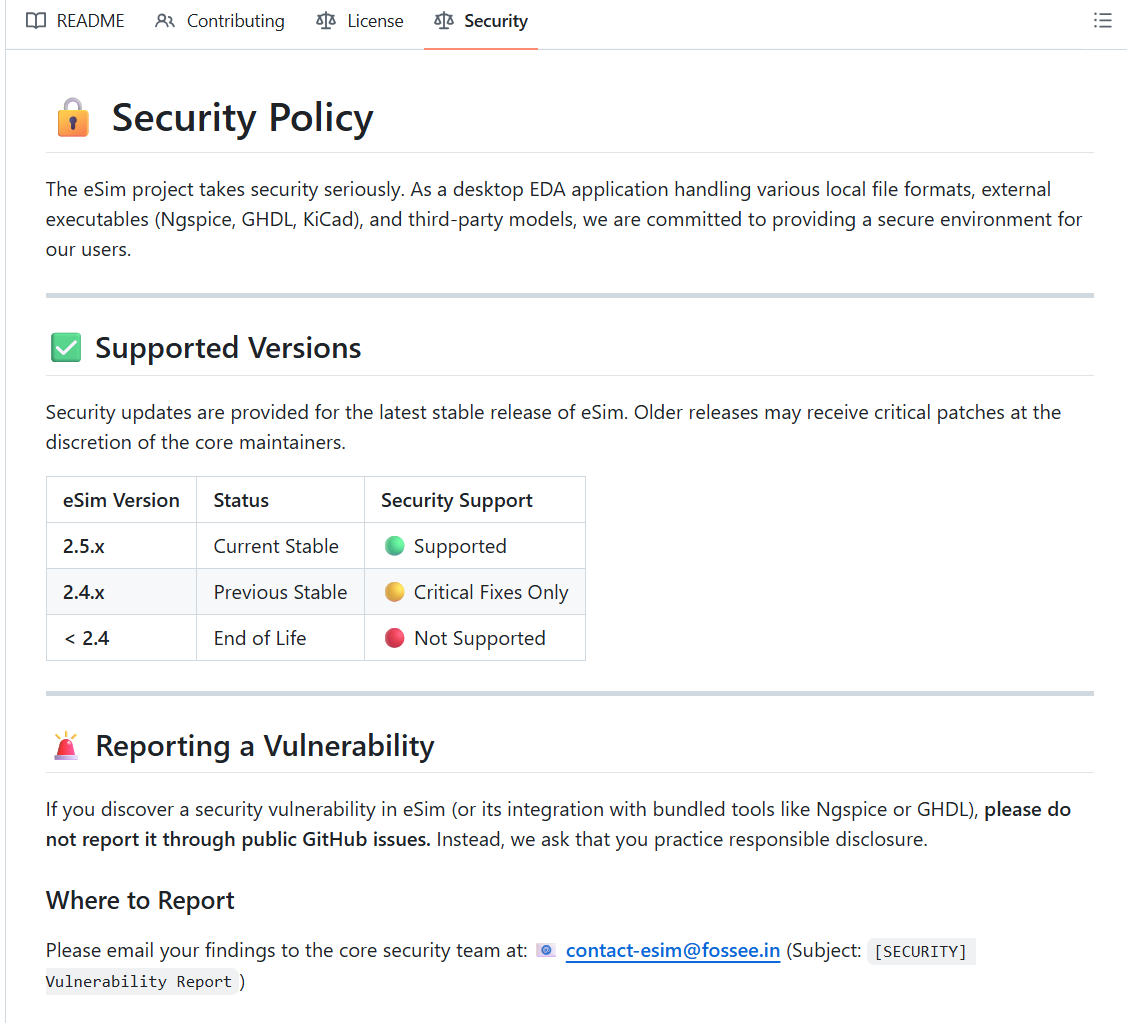
\includegraphics[width=0.9\textwidth]{figures/security_md.png}
    \caption{Screenshot of the enhanced SECURITY.md policy document}
    \label{fig:security_md}
\end{figure}

% ======================================================
% CHAPTER 4: GUI ENHANCEMENTS & CODE REFACTORING
% ======================================================
\chapter{Advanced GUI Enhancements \& Refactoring}
\section{The State of the Existing Interface}
By the time I began my work on the Tool Manager, the core features and the three-tab layout (Quick Setup, Individual Tools, Bulk Uninstall) had already been implemented by other contributors. However, while the functionality was present, the interface itself suffered from severe usability issues and visual inconsistencies. 

Data within the PyQt6 tables was severely congested, layouts broke entirely under different resolutions, and Windows Dark Mode caused severe contrast bleed that rendered entire sections unreadable. My objective was not to build new features, but to meticulously polish, refactor, and enhance the existing UI to bring it up to professional software standards.

\section{Comprehensive UI Polishing and CSS Refactoring}
In my UI/UX enhancement commits (specifically \texttt{9418ef3b} and \texttt{d9ac8a93}), I systematically reviewed the existing implementation and resolved the following layout and styling issues without altering the underlying backend logic:

\begin{itemize}
    \item \textbf{Typography and Spacing:} The original \texttt{ToolManagerGUI} table suffered from text overlapping cell borders. I de-congested the table by increasing row heights, injecting cell padding, and enabling alternating row colors, which drastically improved the readability of complex version strings.
    \item \textbf{Dark Theme Inconsistencies:} On Windows machines with system-wide Dark Mode enabled, PyQt6 inherited dark palettes that clashed violently with hardcoded light elements. This resulted in solid black rendering on the \texttt{UninstallWindow} and progress frames, and a thick black horizontal line below the tab navigation. I fixed this by applying explicit, forced light-themed stylesheets and white backgrounds across the central \texttt{QWidget} and \texttt{QTabWidget}.
    \item \textbf{Modernized Scrolling:} I implemented a modern, customized scroll bar to replace the clunky default OS scrollbars, ensuring smoother navigation through long lists of dependencies.
    \item \textbf{OS-Level Integration:} I integrated the Tool Manager directly into the main eSim Top Toolbar for much quicker developer access, and added a dedicated taskbar icon to improve OS-level window management.
\end{itemize}

\section{Responsive Design Fixes}
One of the most critical issues I faced was the responsive breakage in the Quick Setup tab. When users initiated a long-running installation process, a large progress frame would appear at the bottom of the window. In lower resolution environments, this sudden appearance forced the installation buttons upward, squishing them into an unusable graphical glitch.

To resolve this, I architecturally wrapped the "Quick Setup" tab contents inside a dynamic \texttt{QScrollArea}. This allowed the layout engine to gracefully handle the appearance of the progress frame without distorting or hiding the primary navigation buttons on smaller screens. I applied similar re-spacing and padding fixes to the bottom action buttons across all tabs to maintain a consistently clean layout.

\section{Visual Walkthrough of the Polished Interface}
The culmination of these styling refactors, padding adjustments, and responsive fixes transformed the existing features into a highly polished, user-friendly experience.

\begin{figure}[H]
    \centering
    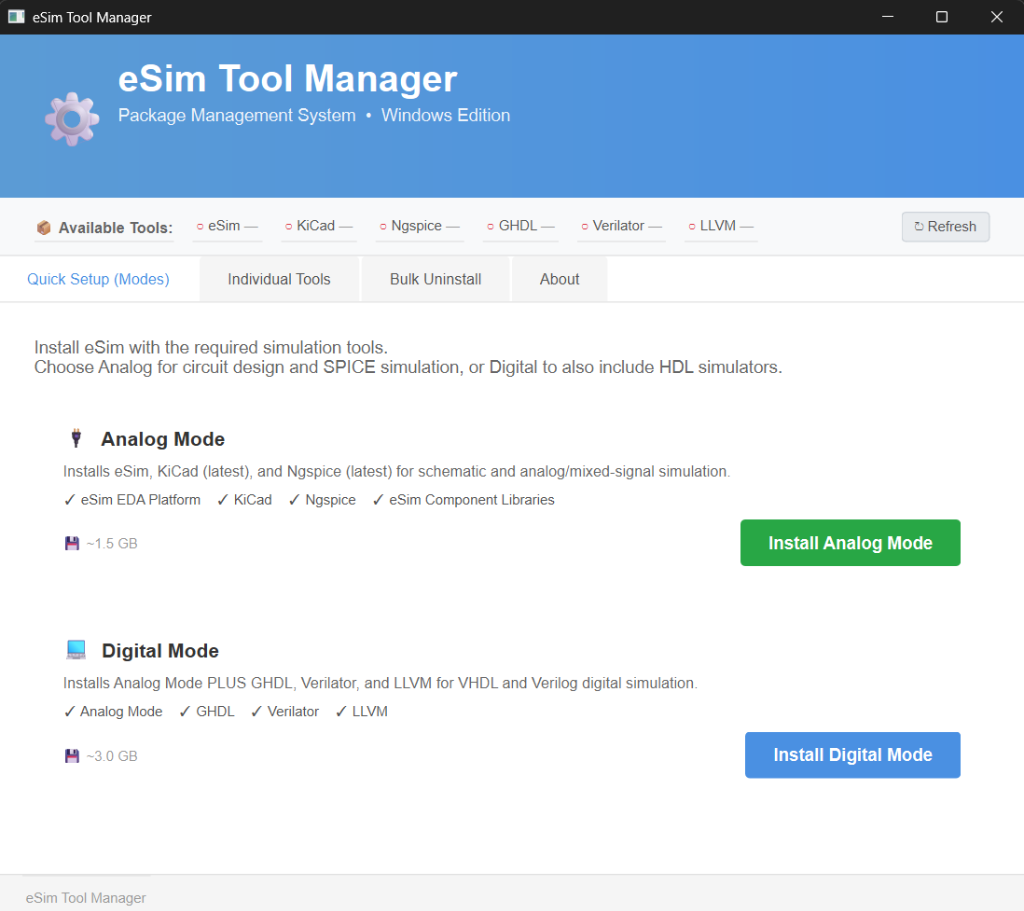
\includegraphics[width=0.65\textwidth]{figures/gui_quick_setup.png}
    \caption{The polished Quick Setup tab, now utilizing a QScrollArea to prevent layout squishing}
    \label{fig:gui_quick_setup}
    
    \vspace{0.3cm}
    
    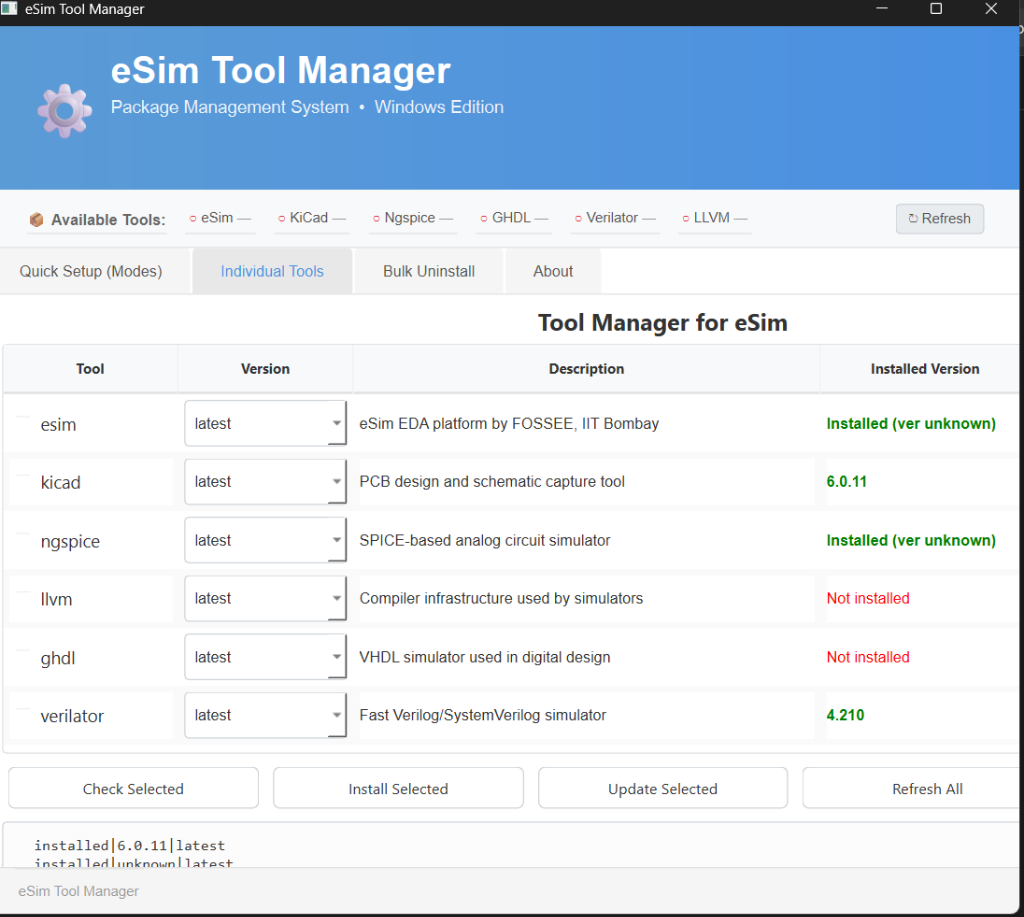
\includegraphics[width=0.65\textwidth]{figures/gui_individual_tools.png}
    \caption{The Individual Tools table, enhanced with proper cell padding and alternating row colors}
    \label{fig:gui_individual_tools}
\end{figure}

\begin{figure}[H]
    \centering
    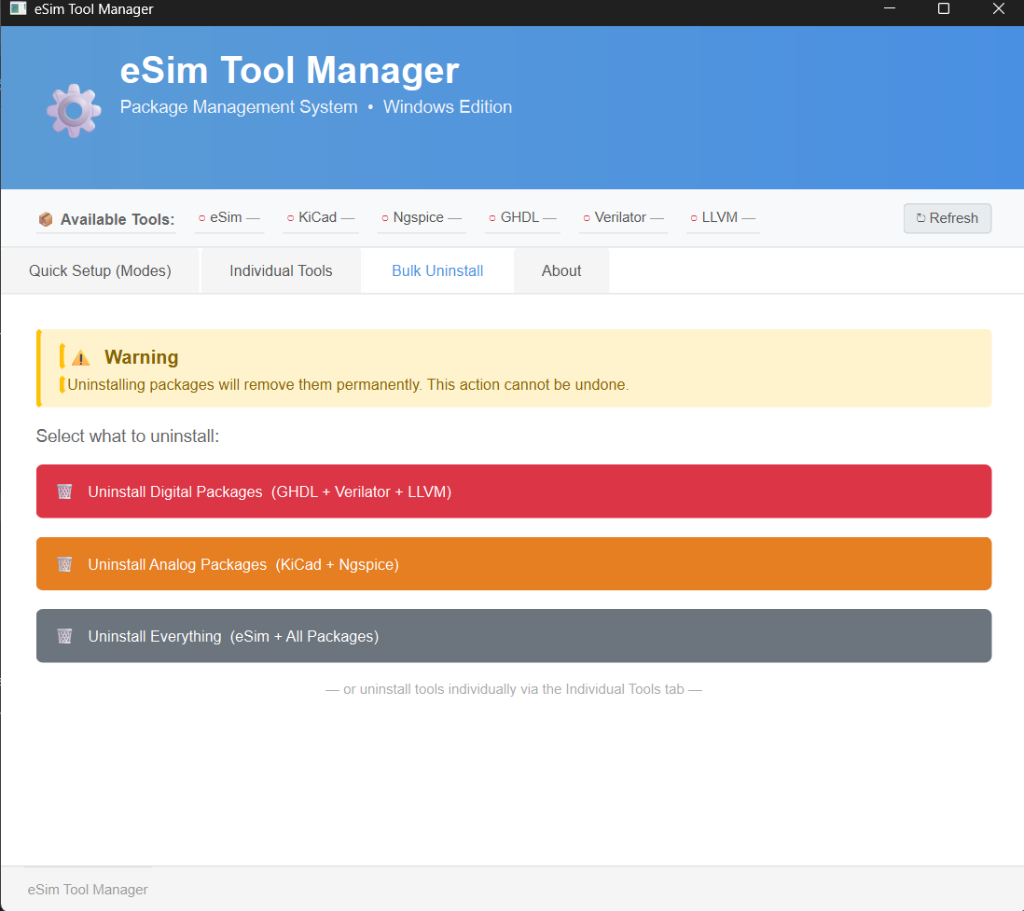
\includegraphics[width=0.65\textwidth]{figures/gui_bulk_uninstall.png}
    \caption{The Bulk Uninstall tab, featuring fixed typography and re-spaced action buttons}
    \label{fig:gui_bulk_uninstall}
    
    \vspace{0.3cm}
    
    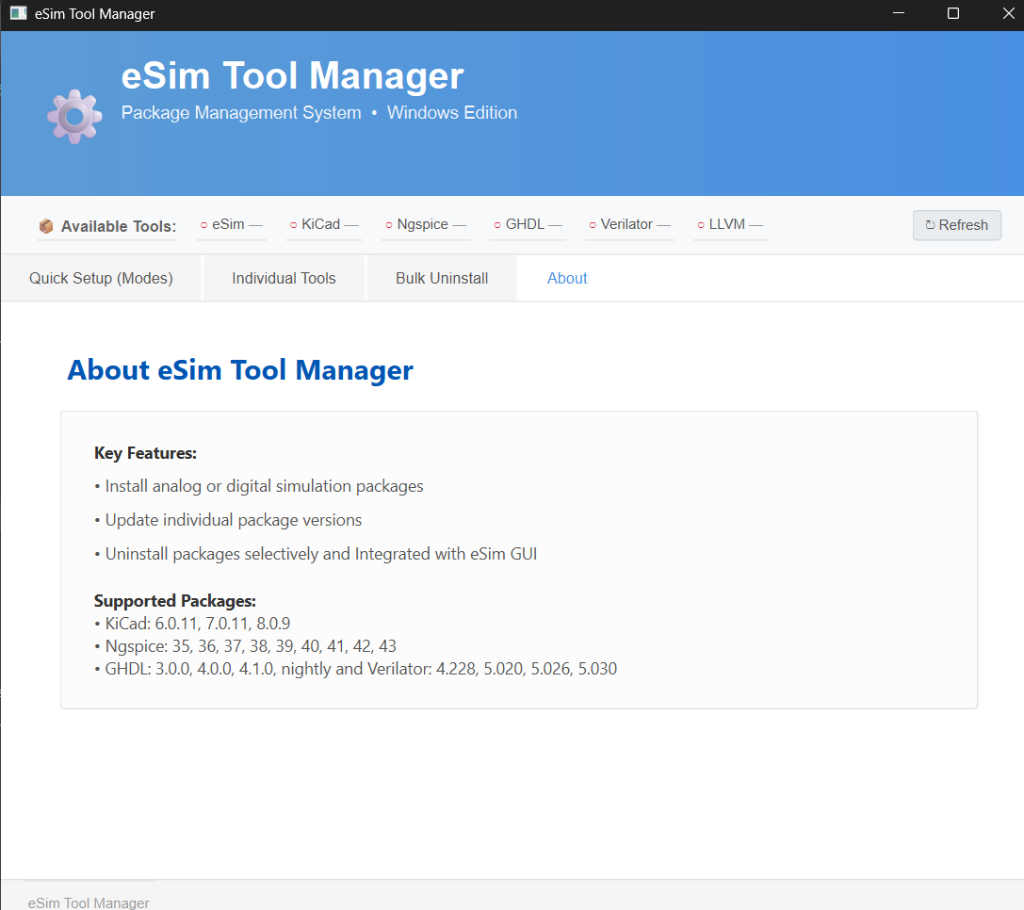
\includegraphics[width=0.65\textwidth]{figures/gui_about.png}
    \caption{The About screen, maintaining consistent light-themed styling without dark mode bleeds}
    \label{fig:gui_about}
\end{figure}





% ======================================================
% CHAPTER 5: MINOR TASK
% ======================================================
\chapter{Minor Task: KiCad Frontend Analysis \& Bug Fixes}
As a minor task during the fellowship, I was assigned to investigate and resolve several outstanding issues within the KiCad frontend interface and its associated backend converters. The KiCad suite forms the backbone of schematic capture in eSim, making its stability paramount for the overall user experience.

With the overarching ecosystem migrating towards newer frameworks, the KiCad frontend was suffering from broken API calls, layout regressions, and path parsing errors. My contributions involved a thorough architectural analysis of the existing Python codebase to identify the root causes of these bugs, followed by implementing targeted fixes.

\section{Debugging the PyQt6 Migration Regressions}
During the transition from PyQt5 to PyQt6, several legacy enumerations and strict type comparisons were left broken in the frontend. Because PyQt6 enforces stricter scoping for Qt enums (e.g., \texttt{Qt.AlignmentFlag.AlignTop} instead of the older \texttt{Qt.AlignTop}), the application would silently throw exceptions or fail to render entirely. I systematically traced the stack traces generated during KiCad parameter dialog instantiation. By mapping out the deprecated API calls and replacing them with their modern PyQt6 equivalents, I ensured that the KiCad interface widgets rendered flawlessly without runtime crashes. This required meticulously updating the \texttt{QAbstractItemView} and various layout manager flags across multiple Python modules.

\section{Path Resolution in kicadToNgspice Converters}
A critical issue was identified in the netlist conversion pipeline. The \texttt{kicadToNgspice} converters occasionally struggled with parsing dynamic file paths, especially on Windows environments where directory trees frequently contain spaces or unusual characters. When KiCad generated a schematic file, the converter would split the path incorrectly, leading to silent failures during the Ngspice simulation phase.

To resolve this, I fortified the path handling logic by implementing robust string parsing and leveraging Python's path management utilities. This ensured that all subcircuit library references and netlist files were safely escaped and parsed regardless of the host operating system. This fix prevented silent conversion failures and restored seamless integration for Windows users.

\section{Dialog Box Alignment and Layout Polish}
Similar to the UI inconsistencies found in the Tool Manager, the KiCad frontend dialogs suffered from overlapping widgets and hardcoded geometry that broke on high-DPI displays. I applied standardized \texttt{QVBoxLayout} and \texttt{QHBoxLayout} constraints, removing absolute positioning. By injecting proper cell padding and layout margins, I guaranteed that the KiCad to Ngspice conversion windows remained clean, readable, and dynamically responsive across all display resolutions.

By systematically analyzing these frontend issues and applying robust structural fixes, I ensured that the KiCad integration remained highly stable. This allows eSim users to seamlessly transition from schematic capture to Ngspice simulation without encountering unexpected UI glitches or data loss.

% ======================================================
% CHAPTER 6: DEPLOYMENT AND VERSION CONTROL
% ======================================================
\chapter{Version Control \& Deployment Workflows}

\section{Commit History and Atomic Operations}
Throughout this fellowship, a strict adherence to atomic commits and semantic versioning was maintained. This practice ensures that GUI refactoring is entirely isolated from documentation updates, allowing project maintainers to bisect bugs efficiently. By following the Conventional Commits specification, the version history remains self-documenting and highly readable for future contributors.

The exact commits authored for these improvements include:
\begin{itemize}
    \item \texttt{d9ac8a93}: \textit{style(tool-manager): polish PyQt6 UI and fix dark theme inconsistencies}
    \item \texttt{9418ef3b}: \textit{feat(ui): implement comprehensive UI/UX enhancements for tool manager}
    \item \texttt{d3eec613}: \textit{docs: comprehensive documentation updates including README, CONTRIBUTING, and SECURITY policies}
\end{itemize}

\section{Branch Management and Code Review}
All feature development, including the KiCad frontend bug fixes and the Tool Manager UI enhancements, was performed on isolated feature branches. These branches were subjected to rigorous local testing across different operating systems (Windows and Linux) before being submitted as Pull Requests (PRs). The PR workflow facilitated detailed code reviews by the FOSSEE maintainers, ensuring that all code met the repository's strict quality standards before merging into the main production branch.

\section{Continuous Integration Integrity}
By confining the GUI enhancements to stylesheet overrides and structural layout wrappers (like \texttt{QScrollArea}), the underlying business logic of the Automated Tool Manager remained untouched. This strategic decision ensured that the existing Continuous Integration (CI) pipelines and automated unit tests passed flawlessly upon integration, as the core \texttt{installer.py} and \texttt{dependency\_checker.py} modules experienced zero friction. Furthermore, the CI pipeline's linting tools seamlessly validated the updated codebase, guaranteeing a stable deployment workflow.

\section{Deployment Workflows and Future Automations}
While the current continuous integration framework validates the codebase successfully, the deployment workflow can be significantly enhanced through advanced GitHub automations. In the future, the repository's deployment pipeline can incorporate fully automated release generation, eliminating the need for manual binary packaging across different operating systems.

Furthermore, future automations can be implemented to dynamically keep the repository's documentation up to date. By leveraging GitHub Actions, the system can automatically extract Python docstrings, generate updated Markdown content, and render fresh Mermaid architecture diagrams upon every merge to the main branch. This means the \texttt{README.md}, API references, and contributor metrics will self-update. Such an automated deployment workflow ensures that the documentation never falls out of sync with the actual software deployment, vastly reducing technical debt without requiring direct human intervention.

% ======================================================
% CHAPTER 7: CONCLUSION AND FUTURE WORK
% ======================================================
\chapter{Conclusion and Future Work}
\section{Conclusion}
The eSim Summer Fellowship 2026 provided a rigorous and technically demanding platform to bridge the gap between core backend functionality and end-user accessibility. Working on an open-source project of this scale offered invaluable insights into software architecture, collaborative version control, and the critical importance of user experience in Electronic Design Automation (EDA) tools.

The comprehensive documentation overhaul transformed the repository from a basic code dump into an inviting, professionally maintained open-source ecosystem. By implementing dynamic Mermaid architecture diagrams, live-fetching contributor statistics, and meticulously structured Markdown guidelines, the onboarding process for new developers has been vastly simplified. This reduction in technical debt has drastically lowered the maintenance overhead for project leads and community moderators.

Simultaneously, the extensive GUI enhancements have fortified the Automated Tool Manager against platform-specific rendering bugs. The strict enforcement of light-themed stylesheets, coupled with mathematically calculated padding and dynamic scroll areas, guarantees that eSim users receive a premium, responsive experience regardless of their hardware or operating system. Fixing the PyQt6 migration regressions within the KiCad frontend further stabilized the core schematic capture workflow, demonstrating the value of deep codebase analysis and atomic refactoring.

These contributions form a critical foundation for the continued scaling of the eSim platform, ensuring it remains at the forefront of open-source EDA initiatives and educational tools globally.

\section{Future Work}
Looking forward, several exciting technical avenues exist to further enhance and modernize the eSim ecosystem:
\begin{itemize}
    \item \textbf{AI-Based Debugging Integration:} Exploring the integration of AI-powered chat assistants directly within the Tool Manager and KiCad frontend. This would assist users with real-time error resolution, suggest netlist fixes, and provide circuit design hints based on common Ngspice compilation errors.
    \item \textbf{Cross-Platform Native Portability \& Containerization:} Expanding the Tool Manager's portability layers to guarantee seamless execution without reliance on local MSYS2/MinGW environments on Windows. Packaging the toolchain via Docker containers or Flatpak could provide true one-click deployments for Linux users.
    \item \textbf{Automated Test Suites and CI/CD Expansion:} While the current integration is stable, building a comprehensive suite of UI tests using tools like \texttt{pytest-qt} would prevent future layout regressions. Expanding the GitHub Actions pipelines to automatically build executable binaries for Windows, macOS, and Linux upon every release tag would streamline the deployment process.
    \item \textbf{Interactive Documentation Generation:} Automating the generation of documentation and Mermaid graphs directly from the Python docstrings via CI/CD pipelines. This would keep architectural diagrams and backend API documentation perfectly synchronized with the evolving codebase without manual intervention.
\end{itemize}

% ======================================================
% BIBLIOGRAPHY
% ======================================================
\addcontentsline{toc}{chapter}{Bibliography}
\begin{thebibliography}{99}

\bibitem{paknikar2021}
R. Paknikar, S. Bansode, G. Nandihal, M. P. Desai, K. M. Moudgalya, and A. Jha, 
\textit{``eSim: An Open Source EDA Tool for Mixed-Signal and Microcontroller Simulations,''} 
2021 4th International Conference on Circuits, Systems and Simulation (ICCSS), Kuala Lumpur, Malaysia, 2021, pp. 212-217.

\bibitem{patil2024}
V. Patil, R. B. Paul, S. Kar, and K. M. Moudgalya, 
\textit{``eSim: An Open-Source EDA Tool for Education,''} 
Workshop on Open-Source EDA Technology (WOSET), 2024.

\bibitem{fosseeesim}
FOSSEE, IIT Bombay. \textit{eSim Official Website}. 
Available online: \url{https://esim.fossee.in/}

\bibitem{esimgithub}
FOSSEE, IIT Bombay. \textit{eSim GitHub Repository}. 
Available online: \url{https://github.com/FOSSEE/eSim}

\bibitem{pyqt6}
Riverbank Computing. \textit{PyQt6 Reference Guide}. 
Available online: \url{https://www.riverbankcomputing.com/static/Docs/PyQt6/}

\bibitem{kicad}
KiCad EDA. \textit{KiCad Documentation}. 
Available online: \url{https://docs.kicad.org/}

\bibitem{ngspice}
Ngspice. \textit{Ngspice User's Manual}. 
Available online: \url{https://ngspice.sourceforge.io/docs.html}

\bibitem{shields}
Shields.io. \textit{Concise, consistent, and legible badges in SVG and raster format}. 
Available online: \url{https://shields.io/}

\bibitem{mermaid}
Mermaid. \textit{Diagramming and charting tool}. 
Available online: \url{https://mermaid.js.org/}

\bibitem{githubactions}
GitHub. \textit{GitHub Actions Documentation}. 
Available online: \url{https://docs.github.com/en/actions}

\bibitem{msys2}
MSYS2. \textit{Software Distribution and Building Platform for Windows}. 
Available online: \url{https://www.msys2.org/}

\end{thebibliography}

\end{document}
